\documentclass[a4paper,10pt]{article}
\usepackage{listings}
\usepackage{graphicx}
\title{\vspace{-1.5em}\textbf{Seminar 3 Green Threads}}
\author{{\textbf{Amirhossein Namazi}} \\
        {\texttt{<anamazi@kth.se>}} \\
        {KTH Royal Institute of Technology}}


\begin{document}
\maketitle

\section*{Introduction}
The main purpose of this seminar was to understand how threads work on the inside. We were required to implement our own thread library. Our thread library will run in the user space instead of the kernel space.This implementation is based on and very similar to \textbf{pthread} library. At the end we will compare our implementation with the \textbf{pthread} library.
\section*{Managing Contexts}
In this part of the seminar we use the \textbf{contexts} to implement our threads. We would need to use some library calls to initialize and make use of contexts such as \textbf{getcontext(), makecontext(), setcontext() and swapcontext()}.
We are going to create some functions that are very similar to the \textbf{pthread} library functions such as \texttt{pthread\_create()}, \texttt{pthread\_yield()} and \texttt{pthread\_join()}.

Our implementation obviously needs to keep track of running threads, suspended threads and terminated threads. To follow the structure of the \textbf{pthread} library we will represent the threads with a structure. This structure will hold all the necessary information for handling the threads such as the pointers, terminated flag, context,... .
To be able to keep track of the suspended and terminated threads, we will implement a queue structure.

\begin{lstlisting}[language=C]

void add_queue(green_t** queue, green_t *thread){
  green_t* current = *queue;
  if(current == NULL){
    *queue = thread;
  }

  else{
    while(current->next != NULL){
      current = current->next;
    }
    current->next = thread;
  }
}

\end{lstlisting}

One of the main problems that I encountered during this part of the assignment was actually handling the queue. It was kind of tricky to work with the\textbf{ \texttt{green\_t}} structure. The queue is implemented as a FIFO queue. we add a thread to the end of the queue of suspended threads and we will get the first thread in the queue to swap the contexts. In addition to that it is also worth mentioning that in our implementation we assume that there is always one thread waiting for another thread. This will make the implementations easier as it prevents undefined behaviour.

After implementing this section and debugging multiple times, I was able to successfully run the simple test.

\section*{Suspending on a condition}
So far in our implementation we use \texttt{green\_yield()} function to suspend the threads which basically puts the running thread last in the ready queue. But another approach is to use the conditional variables. In this approach a thread will sleep until a task is ready.

To be able to write the required functions, we have to define a new data structure \texttt{green\_cond\_t} which would hold a number of suspended threads. The \texttt{green\_cond\_wait()} function will suspend the thread and the \texttt{green\_cond\_siganl()} would take the first suspended thread out of the suspended list and add it to the ready queue.

\section*{Adding a timer interrupt}
So far threads are suspending either by explicitly calling \texttt{green\_yield()} function or using the conditional variables. Since our implementation is in the user space, once could take advantage of this and develop their applications so that they would never suspend. So in order to prevent this and allow the threads to run concurrently we want to have a timer driven scheduling.

After including needed headers, defining macros and completing the code for \texttt{init()} and \texttt{timer\_handler()} we can run a simple test. But some of the tests would result in a segmentation fault. The reason is when we are changing and manipulating a data structure such as a queue and then an interrupt happens, things will not work as intended. So we have to block and unblock the interrupts when we are dealing with these type of situations.

Below is the code that shows threads are suspending without calling \texttt{green\_yield()} function or using the conditional variables but with the timer interrupt.

\begin{lstlisting}[language=C]

void *test(void *arg){
  int id = (int)arg;
  int loop = 10000;
  while(loop > 0){
    printf("thread %d: %d\n", id, loop );
    loop--;
  }
}

\end{lstlisting}

and the output where the threads alternate
\begin{lstlisting}[language=C]
thread 0: 403
thread 0: 402
thread 0: 401
thread 0: 400
thread 0: 399
thread 1: 1152
thread 1: 1151
thread 1: 1150
thread 1: 1149
thread 1: 1148
\end{lstlisting}

A very important issue that I encountered here was how timer interrupts are handled in the Windows Subsystem for Linux. Somehow I couldn't get the threads to run concurrently using timer interrupts which most probably is an issue with WSL since WSL does not have a Linux kernel at all. So I had to ask a friend to run the code for me.

\section*{A Mutex lock}
Different parts of the library are coming together but there are situations where our library falls short. A simple scenario is when two threads increment a shared counter.

\begin{lstlisting}[language=C]

void *testFail(void *arg){
  int id =(int)arg;
  for(int i=0; i < 10000; i++){

    for (int i = 0; i < 2000; i++);

    counter++;
    printf("thread %d: %d %d\n", id, i, counter );
  }
}

\end{lstlisting}
The second for loop in the code is to actually make the process slower so we would catch timer interrupts.

We know that this test will fail and the output further proves our claim since the correct counter value should be 20000.

\begin{lstlisting}[language=C]
thread 0: 9995 19264
thread 0: 9996 19265
thread 0: 9997 19266
thread 0: 9998 19267
thread 0: 9999 19268
Done!
counter:19268
\end{lstlisting}

We can easily fix this problem by having a mutex construct that synchronizes threads. For this, we would have to define a new structure \texttt{green\_mutex\_t} that will hold a list of suspended threads since threads suspend on a lock if it is taken.

After implementing the mutex function, if we now refine the same test that failed so that we take the lock before incrementing the counter and releasing it afterwards, things will work as they should.

\section*{The final touch}
This section is about atomic conditional operations which in our case
is          \texttt{green\_cond\_wait()}. If we do suspending and releasing in two different stages, a thread might try to access the lock right after suspending and right before releasing stages. So it won't get the lock although the lock technically is released.
We then change our implementation for \texttt{green\_cond\_wait()} to release the lock while suspending on a condition.

\section*{Benchmark}
Benchmarks and testing was a difficult and tricky part of this assignment. The main idea behind the becnhmarking was to implement a producer and a consumer to synchronize their actions using conditional variables and mutex locks. In other words, there are two threads which one of them acts as a producer and the other as a consumer. The threads will update a global variable to either 1 if it's a producer and 0 if it's a consumer. Each thread will do this 50000 times. To prevent a race condition we use mutex locks. The conditonal varibales are also used when a thread is wating for another one to finish its task. To be able to compare how well our library perforems we will develop the same test for threads using \textbf{pthreads} library and compare the execution time.

\begin{figure}[htp]
    \centering
    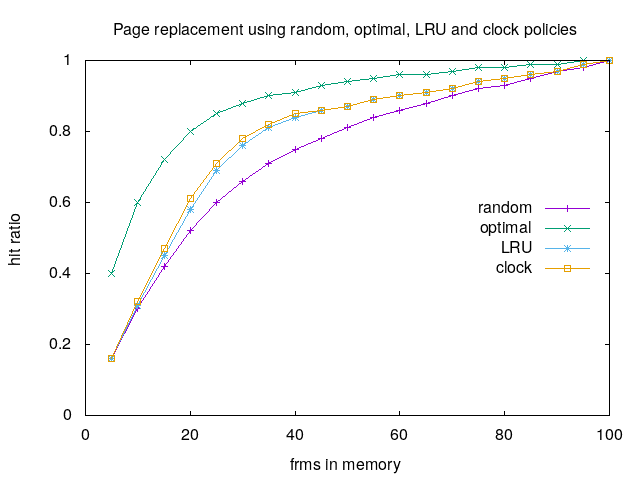
\includegraphics[width=11cm]{graph.jpeg}
    \caption{A comparison between our green library and pthread library}
    \label{fig:graph}
\end{figure}

This is kind of expected from the theoretic point of view since our library is handled in the user space hence should be faster than a library that uses kernel space.
Another important point which is worth mentioning is that this test was ran on an Ubuntu machine. If we run the same test on a WSL, we would get totally different results. In WSL pthread seems to be working faster than our library. Which in my opinion is wrong since WSL only mimics Linux's behaviour and does not have a Linux kernel.

\section*{Conclusion}
This assignment helped me understand how \textbf{Threads} actually work. I learned a lot by implementing a small thread library that is very similar to the \textbf{pthreads} library. One of the things I would like to point out is the issues WSL has when you are dealing with the kernel. So just use a real Linux machine or a virtual machine instead of WSL and make your life easier.

\end{document}
